Al momento de escribir este informe, el código HDL del circuito a someter se puede sintetizar mediante la herramienta Synplify Premier únicamente. Con esta herramienta se escoge para que tipo de tecnología se desea sintetizar el código HDL, la misma genera la Netlist en Verilog del DUT. La Netlist así generada se sitúa en la entrada de MODNET para automatizar el proceso de modificación de las bibliotecas del Xilinx. Algunos de los componentes modificados son los FFD y sus distintos ejemplares (FDC, FDE, etc.) y también las LUTs que incluye las compuertas lógicas y los multiplexores.
La salida de MODNET es la Netlist modificada con  señales extras de entradas usadas para inyectar las fallas en los registros y las compuertas lógicas. De esta manera se logra preparar un RTL para que puedan inyectarse SEUs y SETs. En este sentido, la arquitectura interna original no se cambia y se respeta tal cual es. 


\subsection{Emulación de SEU: Flip-Flops}
En la figura ~\ref{FF} se muestra el extra hardware que se debe agregar para generar un circuito capaz de ser implementado para un futuro proceso de inyecciones. Se puede notar que el extra hardware se limita a un multiplexor, la señal de inyección INJ y una compuerta NOR.
En la figura ~\ref{FFS} se puede ver su comportamiento y cómo  actua en el caso que haya una inyección o en el caso que no la haya. Se muestra que su comportamiento original no se modifica en el caso en que la inyección  no suceda. Es por ello que el cambio es no invasivo y respecta el comportamiento original del circuito.


\begin{figure}[H]
	\centering
	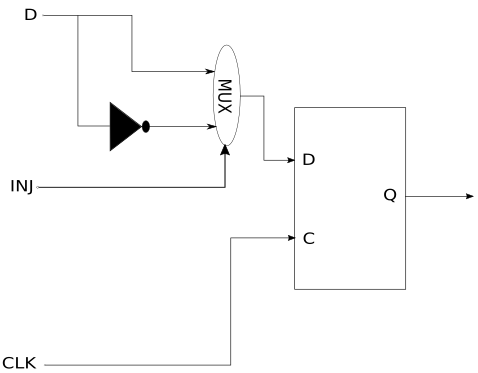
\includegraphics[width=0.55 \textwidth]{img/FF.png}
	\caption{Modificación de un Flip-Flop sin la señal de habilitación}
	\label{FF}
\end{figure}

\begin{figure}[H]
	\centering
	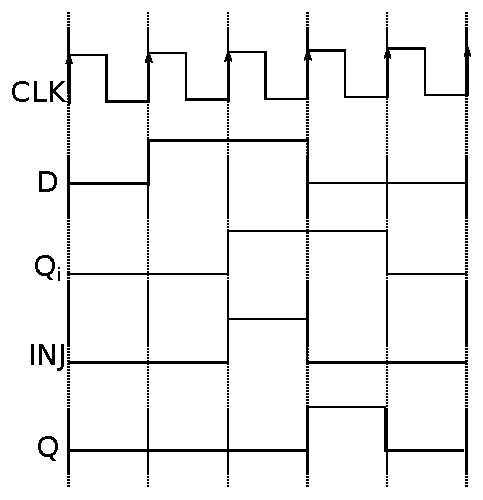
\includegraphics[width=0.48 \textwidth]{img/dessin.pdf}
	\caption{Formas de la onda del FF modificada con  $Q_{i}$ la cual es la salida original sin INJ }
	\label{FFS}
\end{figure}

En la siguiente fracción de  código se puede ver la traducción final en la biblioteca modificada de Xilinx.
\lstset{frame=tb,
  language=VHDL,
  aboveskip=3mm,
  belowskip=3mm,
  showstringspaces=false,
  columns=flexible,
  basicstyle=\ttfamily,
  numbers=none,
  breakatwhitespace=true,
  tabsize=2
}

\begin{lstlisting}

module FDC_mod (inj, Q, C, CLR, D);

parameter INIT = 1'b0;

output Q;

input C, CLR, D, inj;

wire Din;

FDC uut_FDC(.Q(Q),.C(C),.CLR(CLR),.D(Din));

assign Din = (inj) ? !D : D;

endmodule

\end{lstlisting}

Es necesario  aclarar que existen diferentes tipos de modificaciones posibles en los flip-flop las cuales se asemejan más a la realidad dependiendo del tipo de circuito. Podríamos hacer una primera clasificación sobre los FF en FF que se leen, FF que  se escriben o en FF que hacen las dos cosas. Dependiendo del funcionamiento del circuito se utilizará un tipo u otro FF. De esta forma, la biblioteca que define el comportamiento del FF en Xilinx se remplaza por su versión modificada. Ya que puede ser crítico el momento en que llega la señal de inyección, esto puede ocurrir mientras se está escribiendo el circuito o mientras se está leyendo, pudiendo ocasionar un cambio o no. Por ejemplo, si nuestro circuito solo usa FFD sin \textit{enable}, solo nos interesarán las inyecciones en la escritura del FF, pero si fuese un FFDE el cual pose un \textit{enable}, podría ocurrir que se lea  el FFDE y simultáneamente cayese una inyección, quedando el FFDE en un estado inestable, este tipo de problemas se solucionan con  más lógica combinacional, por lo tanto, más hardware extra.

En la figura ~\ref{FFDE} se muestra la descripción esquemática de un FFDE con su lazo para volver  a un estado estable y el extra hardware para el proceso de inyeccion. El FFDE estará activo cuando la suma de INJ y CE sean iguales a 1. Las opciones son  01 ó 10.  


\begin{figure}[H]
	\centering
	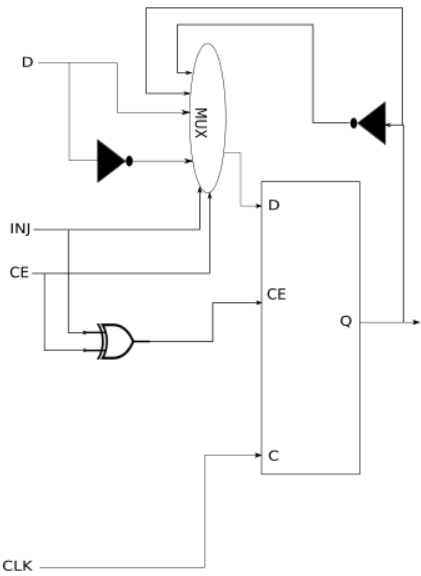
\includegraphics[width=0.5 \textwidth]{img/FFDE.png}
	\caption{Modificación de un FFDE }
	\label{FFDE}
\end{figure}

Por otro lado, en la figura ~\ref{FFDESS}  se puede ver que cuando los estados INJ  y CE son 00 ó 11 el FFDE  no se activa, manteniendo su salida Q.

\begin{figure}[H]
	\centering
	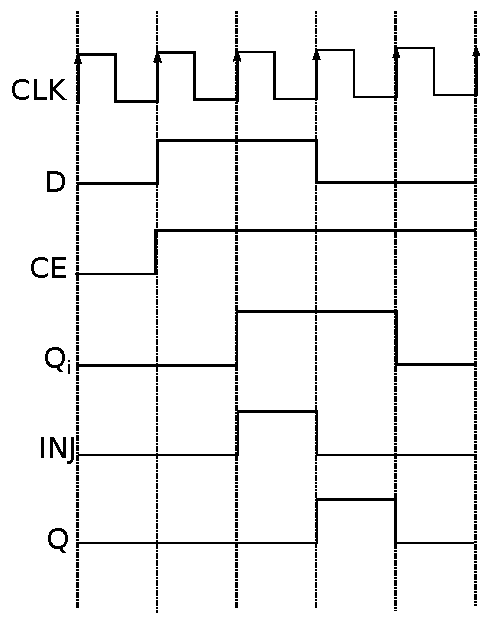
\includegraphics[width=0.4 \textwidth]{img/FFDES.pdf}
	\caption{Comportamiento de un FFDE  modificado }
	\label{FFDESS}
\end{figure}


\subsection{Emulación de SET: Look-Up Table }

Como se menciono anteriormente, luego  de la síntesis con  Synplify Pro, los circuitos  bajo prueba dan como resultado los siguientes tipos de LUTs: LUT4, LUT4\_L, LUT5, LUT5\_L,LUT6, LUT6\_L, a los cuales se le aplica las alteraciones pertinentes para que tengan efecto las futuras inyecciones, tal cual se muestra en la figura \ref{LUT}. En el Anexo A se encuentra el código completo de las librerías que se corresponden a las LUTs original y modificadas.


\begin{figure}[H]
	\centering
	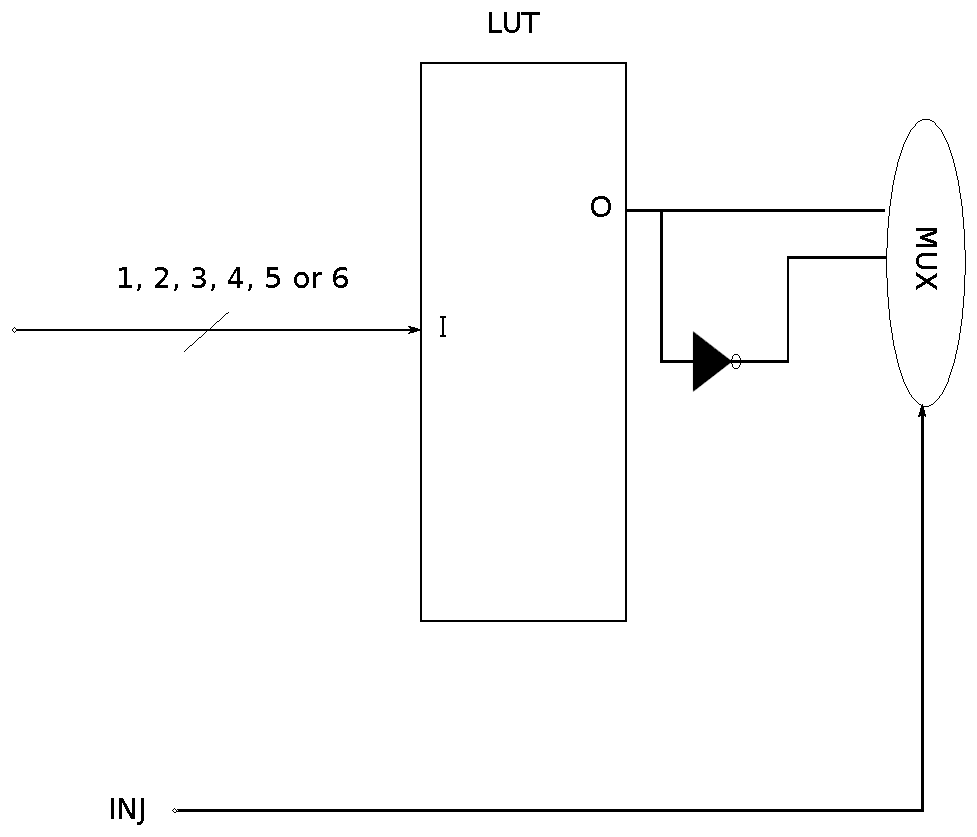
\includegraphics[width=0.4 \textwidth]{img/LUT.pdf}
	\caption{Modificación de una LUT}
	\label{LUT}
\end{figure}


Traducido a código una LUT, independientemente del tipo, a la biblioteca que la define solamente se le agrega  un multiplexor a la salida, el cual será controlado por una señal de inyección. 
\begin{lstlisting}
  module LUT6_L (inj_c,LO, I0, I1, I2, I3, I4, I5);

  parameter INIT = 64'h0000000000000000;

  input inj_c,I0, I1, I2, I3, I4, I5;

  output LO;

  reg LO1;
  reg tmp;
  
  assign LO = (!inj_c) ? LO1 : !LO1;
\end{lstlisting}

En el extracto de código anterior se intenta mostrar que independientemente de la arquitectura que tenga cada LUT, si ocurriese una falla, la salida será la negación del valor correcto de la LUT, determinada por la condición de decisión la cual se implementa en el circuito con un simple  multiplexor.
